\documentclass{ethz_report}
\usepackage{listings}
\usepackage{color}
\usepackage{caption}
\usepackage{subcaption}


\definecolor{codegreen}{rgb}{0,0.6,0}
\definecolor{codegray}{rgb}{0.5,0.5,0.5}
\definecolor{codepurple}{rgb}{0.58,0,0.82}
\definecolor{backcolour}{rgb}{1,1,1}

\lstdefinestyle{mystyle}{
    backgroundcolor=\color{backcolour},
    commentstyle=\color{codegreen},
    keywordstyle=\color{magenta},
    numberstyle=\tiny\color{codegray},
    stringstyle=\color{codepurple},
    basicstyle=\ttfamily,
    breakatwhitespace=false,
    breaklines=true,
    captionpos=b,
    keepspaces=true,
    numbers=left,
    numbersep=5pt,
    showspaces=false,
    showstringspaces=false,
    showtabs=false,
    tabsize=4,
    frame=lines
}
\lstset{style=mystyle}

\title{Exercise 5 - Shape from Silhouettes}
\subject{Computer Vision}
\author{Alberto Montes}
\email{malberto@student.ethz.ch}
\date{\today}

\begin{document}
\maketitle

\section*{Silhouette extraction}

The first task consists on setting the best threshold to extract the image silhouette. With the given images, the best threshold found was $100$ which extract all the figure including the darkest zones because of shadows. It also extract some other places of the environment, but with the bounding box, the noisy extracted parts disappear. On Figure~\ref{fig:silhouette_extraction} there a snapshot of the silhouette extraction.

\begin{figure}[H]
    \centering
    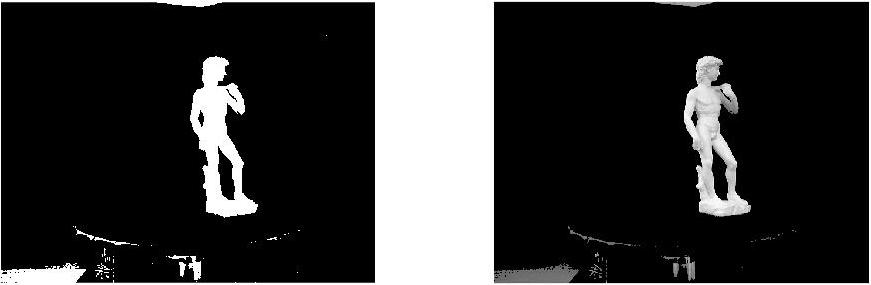
\includegraphics[width=1\linewidth]{images/silhouette_extraction}
    \caption{Silhouette extraction}
    \label{fig:silhouette_extraction}
\end{figure}

\section*{Volume of interest}

Once the silhouette is extracted, it is required to specify the bounding box that will define the volume of interest for the computation of the Visual Hull.
After some iterations, the final values for the bounding box to fit the object has been:

\begin{equation}
    \begin{bmatrix}
        x_{min} & y_{min} & z_{min} \\
        x_{max} & y_{max} & z_{max}
    \end{bmatrix}
    =
    \begin{bmatrix}
        0 & -0.5 & -2 \\
        2.5 & 2 & 3
    \end{bmatrix}
\end{equation}

On Figure~\ref{fig:volume_of_interest} there is a snapshot of the bounding box represented over the silhouette.

\begin{figure}[H]
    \centering
    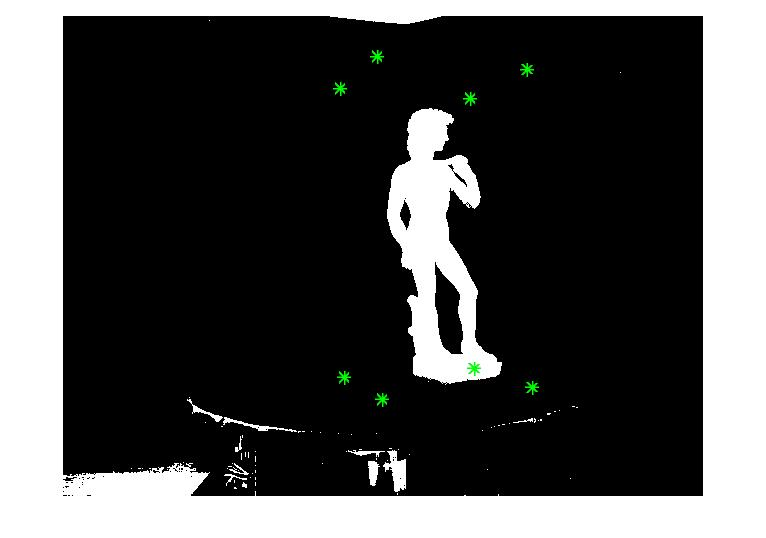
\includegraphics[width=.5\linewidth]{images/volume_of_interest}
    \caption{Volume of Interest}
    \label{fig:volume_of_interest}
\end{figure}

\section*{Visual Hull}

The final step to achieve a 3D reconstruction of the original object at the images, is to compute the Visual Hull. To do so, it has been divided the bounding box into discrete voxels. Then, for each of the voxels, it has been computed the projection of this voxel into each of the captured image and compute in how many images, the voxel is projected into the silhouette. Finally all the voxels with at least \texttt{thresholdVolume} are considered as iso-surface and recreate the original object in 3D.

The implementation of this task is on Listing~\ref{lst:compute_visual_hull} and a pair of details has been taken into account. The first one is that for each voxel it has been computed the projection of the mid point of the voxel, reason why on line \texttt{12}, on each axis is substracted $0.5$. The other detail is taking into account the case where the projected 3D points lays out of the 2D image. In this case we have to ensure the continuity of the program execution.

\lstinputlisting[language=MATLAB, caption=computeVisualHull, firstline=79, lastline=103, label={lst:compute_visual_hull}]{../code/exercise5.m}

The results of the iso-surface are plot on Figure~\ref{fig:visual_hull} where different resolutions have been used for dividing the volume of interest.
In the first case (with a lower resolution) it can be seen how the arms and one leg are not distinguishable and the quality is improvable.
On the other hand, increasing the resolution of the volume of interest, it can be observed a well defined object, with a very similar shape in comparison to the original.

\begin{figure}[H]
\centering
\begin{subfigure}[b]{.5\textwidth}
  \centering
  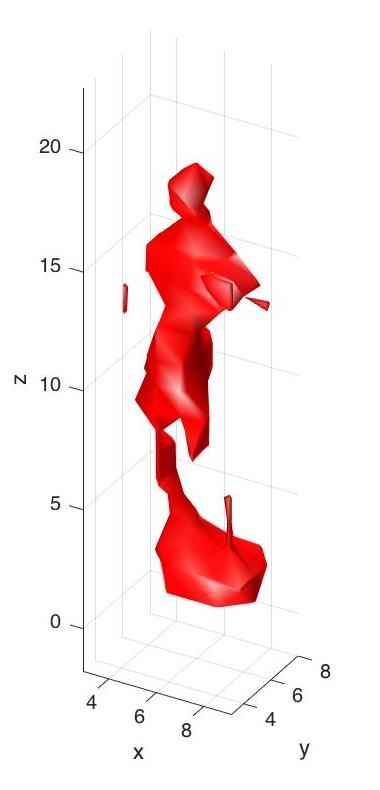
\includegraphics[width=.7\linewidth]{images/visual_hull_low}
  \caption{Volume size: $(10, 10, 20)$}
\end{subfigure}%
\begin{subfigure}[b]{.5\textwidth}
  \centering
  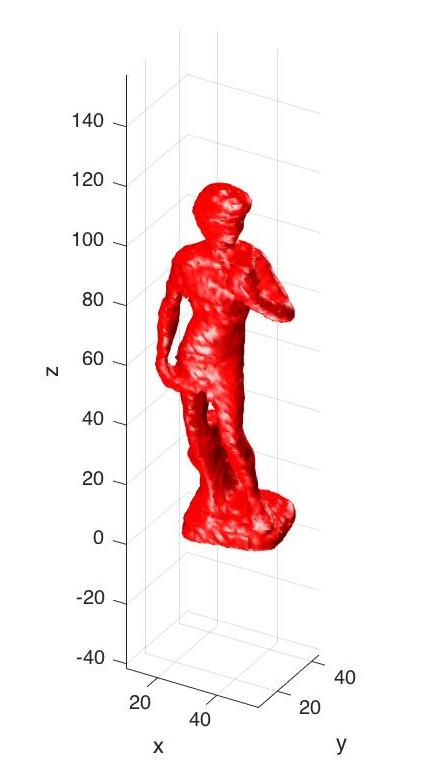
\includegraphics[width=.8\linewidth]{images/visual_hull_high}
  \caption{Volume size: $(64, 64, 128)$}
\end{subfigure}
\caption{Visual Hull for different resolutions}
\label{fig:visual_hull}
\end{figure}

\section*{Improvements}

The method that it has been already implemented consist from a set of images from different angles to the same object reconstruct its 3D model.
To do so, first the silhouette of the object is extracted from each image captured.
Then knowing the projection matrix of each camera, and a bounding box around the object, the bounding box is converted into voxels and each one is projected to each of the images with the silhouettes.
If the voxel lie inside the silhouette for more images than a threshold, this voxel is considered as part of the volume.
Doing so it is possible to find the 3D model finding all this voxels that lie inside enough silhouettes.

This method has the little problem that if the surface of the original object has concave surface, then this method won't be able to correctly identify.

In order to improve this method it can be exploited more information given by the images. This information is referring to the texture of the object. To exploit this information, at the time to compute the visual hull with the silhouettes, when a voxel is projected inside a silhouette, the color value of the projection at the image can be stored, and at the end, for each voxel compute the mean color value and plot it when representing the 3D model.

\end{document}
